% arara: xelatex: { shell : yes }
% arara: biber
% arara: xelatex: { shell : yes }
% arara: xelatex: { shell : yes }

% options:
% thesis=B bachelor's thesis
% thesis=M master's thesis
% Czech thesis in Czech language
% Slovak thesis in Slovak language
% English thesis in English language
% hide links remove color boxes around hyperlinks

\documentclass[thesis=M,czech,hidelinks]{template/FITthesis}[2019/12/23]

\usepackage[utf8]{inputenc} % LaTeX source encoded as UTF-8
\usepackage{dirtree} %directory tree visualization

\usepackage{lipsum}
\usepackage{xevlna}
\usepackage{pdfpages}
\usepackage{minted}
\usemintedstyle{friendly}


\usepackage{chngcntr}
\counterwithin{listing}{chapter}

\usepackage[htt]{hyphenat}
\usepackage{caption}

\usepackage[style=iso-numeric]{biblatex}
\addbibresource{ref.bib}

\usepackage{float}
\usepackage{todonotes}

% \usepackage{siunitx}
% \sisetup{
%     output-decimal-marker={,}% just uncomment if you want to use comma as the decimal marker!
% }


\usepackage{xpatch,letltxmacro}
\LetLtxMacro{\cminted}{\minted}
\let\endcminted\endminted
\xpretocmd{\cminted}{\RecustomVerbatimEnvironment{Verbatim}{BVerbatim}{}}{}{}
\usepackage{csquotes}

\usepackage{xcolor} 
\newcommand{\dummytext}[1]{\textcolor{gray}{\lipsum[#1]}}

\newcommand{\customtodo}[1]{\todo[color=red]{TODO: #1}}

\newcommand{\question}[1]{\todo[color=orange]{Otázka: #1}}

\newcommand{\note}[1]{\todo[color=green]{Pozn.: #1}}

\newcommand{\inlinecode}[1]{\texttt{#1}}

\newcommand{\sourcedcaption}[2]{\caption[#1]{#1. #2}}

\newcommand{\source}[1]{\caption*{{#1}}}

\newcommand{\highlight}[1]{\textcolor{orange}{#1}}

\newcommand{\cpp}{C\nolinebreak[4]\hspace{-.05em}\raisebox{.4ex}{\tiny{\textbf{++}}}}

\newcommand{\csharp}{C\nolinebreak\hspace{-.05em}\raisebox{.45ex}{\tiny{\textbf{\#}}}}


\usepackage{array}
\newcolumntype{L}[1]{>{\raggedright\let\newline\\\arraybackslash\hspace{0pt}}m{#1}}
\newcolumntype{C}[1]{>{\centering\let\newline\\\arraybackslash\hspace{0pt}}m{#1}}
\newcolumntype{R}[1]{>{\raggedleft\let\newline\\\arraybackslash\hspace{0pt}}m{#1}}

% \newcommand{\koruna}[1]{\num[group-minimum-digits=4]{#1}\,{}Kč}
\newcommand{\koruna}[1]{#1\,{}Kč}

\newcolumntype{?}[1]{!{\vrule width #1}}


% % % % % % % % % % % % % % % % % % % % % % % % % % % % % % 
% ODTUD DAL VSE ZMENTE
% % % % % % % % % % % % % % % % % % % % % % % % % % % % % % 

\department{Katedra softwarového inženýrství}
\title{Automatizace testů průmyslové komunikace ve virtualizovaném prostředí}
\authorGN{Martin} %(křestní) jméno (jména) autora
\authorFN{Štěpánek} %příjmení autora
\authorWithDegrees{Bc.\,{}Martin Štěpánek} %jméno autora včetně současných akademických titulů
\author{Martin Štěpánek} %jméno autora bez akademických titulů
\supervisor{Ing.\,{}Daniel Kubeš}
\acknowledgements{\todo{Doplnit}}

\abstractCS{
    Tato diplomová práce se zabývá analýzou, návrhem a implementací rozšíření existující testovací knihovny, která automatizuje testy verifikace průmyslové komunikace. Nová testovací knihovna implementuje integraci virtualizačního řešení Docker, za pomocí než je následně schopna spouštět virtualizovaná průmyslová zařízení a propojit je v různých topologiích. Součástí práce je demonstrace použití a celkové zhodnocení vytvořeného řešení. 
} 

\abstractEN{
    This master's thesis is focused on analysis, design and implementation of extension to the existing testing library, which automates tests that verify industry fieldbus communication. New testing library implements virtualization solution Docker, which enables the library to run virtualized industry devices and connect them in numerous topologies. This thesis also includes demonstration and evaluation of the created solution.
}

\keywordsCS{softwarové testování, automatizace testů, testovací knihovna, verifikace průmyslové komunikace, virtualizace, Docker}
\keywordsEN{software testing, test automation, test library, verifycation of fieldbus communication, virtualization, Docker}

\placeForDeclarationOfAuthenticity{V~Praze}
\declarationOfAuthenticityOption{1} %volba Prohlášení (číslo 1-6)
% \website{http://site.example/thesis} %volitelná URL práce, objeví se v tiráži - úplně odstraňte, nemáte-li URL práce

\begin{document}

\begin{introduction}
V dnešní době softwarového vývoje je podstatné kontinuálně, tedy co nejčastěji, testovat vyvíjený produkt. Na otázku proč co nejčastěji je jednoduchá odpověď. Čím dřív nalezneme daný problém v softwaru, tím rychleji ho můžeme lokalizovat a opravit. Dřívější objevení zároveň většinou znamená menší objem kódu, ve kterém musíme zdroj chyby hledat.

K splnění těchto požadavků je hojně používaná automatizace testů. Díky automatizaci jsme schopni testovat mnohem častěji než manuálně a zároveň minimalizujeme faktor lidské chyby při manuálním testování. Firmy proto často investují nemalé peníze do automatizace testů a jako každý ziskový subjekt, se snaží svoje zisky zvyšovat snižováním vlastních nákladů. 

Jak tedy může firma snížit svoje náklady na testování? Jedna z možností je snaha snížit počet zúčastněných fyzických zařízení. Každé fyzické zařízení musí být zakoupeno a musí být spravováno. Zároveň každé zařízení může v industriálním prostředí existovat v různých konfiguracích. To též musí být otestováno, proto pokud chceme automaticky testovat různé konfigurace, tak poté musí existovat různé sestavy v různých konfiguracích. 

A jak tento problém vyřešit? Jednou možností, je virtualizace testovacích zařízení a topologie zapojení těchto zařízení. Díky virtualizaci jsme schopni simulovat různá zařízení v různých počtech. Cena přidání nového zařízení jsou pouze nutné výpočetní zdroje na zařízení, na kterém testování běží. Dostatečné výkonné zařízení může samozřejmě stát nemalé finance, ale toto zařízení je univerzálnější a znovu použitelné pro všechny produkty, které podporují virtualizaci.

\customtodo{Doplnit obsah kapitol}
\end{introduction}

\chapter{Cíl práce}\label{chap:cil}

Cílem této práce je úprava a rozšíření stávající testovací knihovny, která automatizuje testy verifikace průmyslové komunikace, o virtualizační prvky, díky kterým bude možné za využití knihovny testovat zařízení ve virtualizovaném prostředí. Součástí by měla být i analýza, dle které bude zvolena nejvhodnější možnost implementace testovací knihovny.

Výhodou nově implementovaného rozšíření by měla být nezávislost na externích zařízeních/hardwaru a možnost simulace různých síťových topologií bez nutnosti fyzického zásahu do reálné sítě.

Jednotlivé úkoly tedy jsou:
\begin{enumerate}
    \item Analyzovat způsoby, kterými lze knihovnu rozšířit o virtualizační prvky a zhodnotit je. Knihovna by měla být schopna simulovat různé síťové uspořádání a také by měla být schopna ovládat/vytvářet virtuální testovací partnery. Součástí by měla být také analýza možnosti propojení virtuálních testovacích partnerů se skutečnou sítí.
    \item Dle výstupu z analýzy navrhnout a implementovat řešení, díky čemuž bude testovací služba schopna
          \begin{enumerate}
              \item samostatně spouštět všechny virtualizované účastníky testu,
              \item vytvářet a nastavovat virtuální síť dle zvolené topologie. Testovací služba by měla podporovat sériovou topologii, topologii hvězdy a topologii kruhu.
          \end{enumerate}
    \item Navrhnout a implementovat způsob, kterým bude možné zaznamenávat komunikaci mezi vybranými zařízeními.
    \item Demonstrovat funkcionalitu řešení a zhodnotit vlastnosti implementovaného řešení. Součástí by měla být i diskuze nad reálným využitím daného řešení.
\end{enumerate}

\chapter{Teoretická část}\label{chap:teorie}


\section{Virtualizace}

Koncept virtualizace se poprvé objevil na konci 50.\,let minulého století, kdy skupina z University v Manchesteru vytvořila první funkční prototyp virtuální paměti. Následně v 60.\, letech minulého století byl koncept rozšířen i na celé počítače. První tzv. \textit{virtual machine} (VM), neboli česky \uv{virtuální stroj}, byl vytvořen firmou IBM a jejich cílem bylo umožnit souběžný přístup k sálovým počítačům. Každá VM byla instancí fyzického stroje a dávala iluzi toho, že uživatel přistupuje přímo k fyzickému stroji. Uživatelé mohli vyvíjet, spouštět a testovat aplikace bez obavy toho, že by mohli zhroutit celý počítač, díky tomu, že každá VM byla izolovaná kopie systému. 

Polovinou 70.\,let minulého století byla virtualizace dobře akceptovaným konceptem mezi uživateli. Použitím virtualizace totiž mohli vyřešit podstatné problémy této doby. Například díky již zmíněné virtualizované paměti mohli uživatelé adresovat mnohem větší operační paměť, než počítač skutečně obsahoval. 

Všechny tyto virtualizační techniky byly primárně cesta k vyrovnání se s vysokou pořizovací cenou hardwaru v této době. Díky ní mohli majitelé sálových počítačů využít svoji investici co nejefektivněji. Její použití se tedy se snižujícími cenami hardwaru začalo snižovat a dokonce skoro vymizelo během 80. a 90.\,let díky příchodu levnějších osobních počítačů.  

Poptávka po virtualizaci začala znovu růst až v 90.\,letech minulého století. Se zvětšující se různorodostí hardwaru a softwaru zde vznikla poptávka na to, aby bylo možné spustit aplikace, které původně byly určeny pro jiný hardware a jiný operační systém, na jednom určitém stroji. Poptávka se ovšem zvětšila i v komerčním sektoru. Se zvyšujícími počty serverů firmy hledaly způsoby, jak využít investici do serveru naplno. Spustit pouze jednu aplikaci na serveru nebylo příliš ekonomické, jelikož tato aplikace nemusela vždy využít všechny výpočetní zdroje, a nákup dalších serverů přinášel mimo samotné pořizovací ceny i další náklady, například na údržbu. Řešení pro tento problém tedy byla opět virtualizace. Oba tyto trendy pokračují do dnes a jsou jedny z hlavních důvodů pro použití virtualizace. 

Virtualita se od reality liší pouze ve formálním světě. Má ovšem podobné jádro nebo efekt. V počítačovém světě, virtualizované prostředí je aplikací vnímáno stejně jako reálné prostředí, i když některé mechanismy v něm mohou fungovat jinak. Virtualizované prostředí hlavně dává aplikaci zkreslený obraz reálného stroje, kde v tomto zkresleném obraze může stroj mít více, či méně určitých zdrojů. Typický moderní počítač využívá spoustu takovýchto přístupů. Jedním příkladem je již zmíněná virtuální paměť, díky čemuž může proces použít mnohem více paměti, než je fyzicky dostupné. Tato virtuální paměť taktéž umožňuje sdílení fyzické paměti mezi stovkami procesy. Podobným konceptem je i multitasking, kde jeden procesor je rozdělen a prezentován jako \uv{virtuální procesor} jednotlivým procesům. Na opačné straně, několik procesorů může být seskupeno do jednoho výkonnějšího virtuálního procesoru.

Možností virtualizace je tedy spousta na mnoha úrovních. Virtualizaci tedy můžeme nadefinovat takto:

\begin{displayquote}
    Virtualizace je technologie, která kombinuje/rozděluje, výpočetní zdroje k prezentaci jednoho či více prostředí za pomoci metodologií jako hardwarového a softwarového rozdělování/agregování, parciální/kompletní simulací stroje, emulace a spousty dalších.
\end{displayquote}

Jak je z definice vidět, virtualizace není jenom o rozdělování výpočetních zdrojů, ale o jejich sjednocování do větších celků. V rámci této práce se ale zaměřím primárně na rozdělování výpočetních zdrojů za pomoci virtualizace. Mezi praktické využití virtualizace může patřit například:

\begin{description}
    \item[Konsolidace serveru] Za pomoci virtualizace lze přerozdělit práci z více serverů, které nejsou na plno používány, na jeden server a tím ušetřit na hardwaru, managmentu a administraci infrastruktury. Díky ní tedy snižujeme komplexitu administrace, jelikož všechen software ve VM je nezávislý na softwaru fyzického serveru. 
    \item[Sandbox] Za pomoci virtualizace lze vytvořit bezpečné a hlavně izolované prostředí pro běh aplikací, jejich původ nám může být neznámý a spuštění v normálním počítače by mohlo představovat bezpečnostní riziko. Tato technika se označuje jako \textit{sandboxing}.
    \item[Virtuální hardware] Virtualizace může zprostředkovat hardware, který počítač nikdy neměl. Mezi ně patří například virtuální ethernetové adaptéry, switche, huby atd.
    \item[Spuštění více OS] Bez virtualizace nejsme schopni spustit více operačních systémů zároveň. Virtualizace tedy přináší prostředky, jak toto umožnit. Mimo to ale také přináší prostředky, jak spustit staré operační systémy na novém hardwaru, pro který operační systém nemusel být vyvinut.
    \item[Testování/QA] S pomocí virtualizace jsme schopni vytvořit libovolné testovací scénáře, které jinak mohou těžké vytvořit v reálném světě, čímž může usnadnit testování. 
\end{description}

Jak je vidět z jenom z tohoto krátkého seznamu, důvodů proč virtualizovat existuje spousta. Jak ale virtualizace funguje? V praxi je virtualizace abstrakční vrstva, která poskytuje potřebné propojení mezi dvěma izolovanými vrstvami. Toto si lze lépe představit pomocí obrázku \ref{fig:pc_stack}, na kterém je vidět zjednodušená architektura počítače. Je zde vidět, že virtualizační vrstvu lze vložit mezi jakékoliv dvě vrstvy a tím docílit virtualizace. \cite{campbell2006introduction}\cite{chiueh2005survey}

\begin{figure}[htbp]
    \centering 
    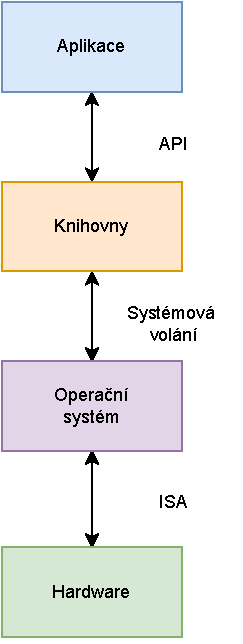
\includegraphics[width=0.325\textwidth]{assets/img/computer_stack.pdf}
    \caption{Architektura počítače ukazující příležitosti k virtualizaci}
    \source{Vytvořeno dle předlohy z \cite{chiueh2005survey}}
    \label{fig:pc_stack}
\end{figure}



\subsection{Možnosti virtualizace}

Jak jsem již nastínil, virtualizační vrstva může existovat na více úrovních. V této sekci bych rád přiblížil virtualizace od nejnižší vrstvy až po tu nejvyšší.

\subsubsection{Virtualizace na úrovni ISA}

ISA, neboli \textit{Instruction Set Architecture} je součástí abstraktního modelu počítače a definuje, jak může software ovládat procesor. ISA funguje jako rozhraní mezi hardwarem a softwarem a specifikuje, co a jak je procesor schopen udělat.\,\cite{isa-arm}

Virtualizace na této úrovni tedy funguje za pomoci softwarové emulace ISA dané platformy. Tedy virtuální vrstva musí být schopna přeložit ISA instrukce hosta na na ISA instrukce hostitele. Tento způsob lze označit i jako \textit{binární překlad}. Tato virtualizace funguje pouze v případě, že existuje způsob, jak na hostitelské platformě provést všechny úkony, požadované architekturou hosta. 

Výhodou této virtualizace je, že nám teoreticky dokáže dát dostatečné prostředky ke spuštění jedné platformy (jako například x86) na ostatních platformách. Taktéž jsme schopni spustit operační systémy, bez žádné modifikace. Tato portabilita ovšem přichází s nemalou cenou. Tím, že musíme každou instrukci softwarově přeložit, tak dochází k velkému snížení výkonu systému. I tak si tento způsob virtualizace nalezne využití. 


\subsubsection{Virtualizace na úrovni HAL}
\customtodo{Vysvětlit co je HAL}

Virtualizace na HAL tedy využívá podobností mezi architekturou platformy hosta a hostitele, díky čemuž může snížit latency způsobenou překladem. Důležitou komponentou v tomto případě je tzv. \textit{hypervizor} (někdy taky označován jako Virtual Machine Monitor - VMM). Hypervizor je softwarová vrstva, která virtualizuje všechny potřebné zdroje fyzického stroje, a tím definuje a podporuje běh jednoho či více VM. \cite{whitaker2002denali}

Existují dva typy hypervizorů. Ty můžeme vidět na obrázku \ref{fig:vm_types}. Hypervizor typu I běží přímo nad hardwarem a spravuje všechny virtuální stroje.

\cite{chiueh2005survey}\cite{RODRIGUEZHARO2012267}

\begin{figure}[htbp]
    \centering 
    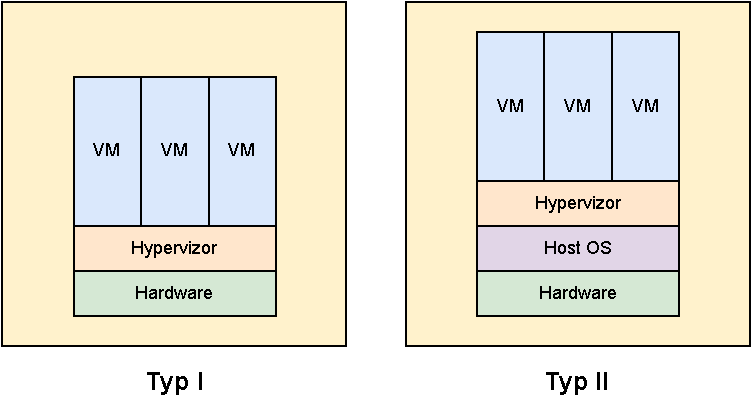
\includegraphics[width=\textwidth]{assets/img/vm_types.pdf}
    \caption{Možné typy virtualizace na úrovni HAL}
    \source{Vytvořeno dle předlohy z \cite{RODRIGUEZHARO2012267}}
    \label{fig:vm_types}
\end{figure}


\subsubsection{Virtualizace na úrovni operačního systému}


\subsubsection{Virtualizace na úrovni programovacího jazyku}


\subsubsection{Virtualizace na úrovni knihoven}



\chapter{Analytická část}\label{chap:anal}

V této kapitole se budu věnovat analýze aktuálního stavu testovací knihovny a možnostech jejího rozšíření.


\section{Analýza stávajícího stavu knihovny}

Původní testovací knihovna byla výstupem mojí bakalářské práce\cite{bakalarka} dokončené v roce 2021. Cílem této knihovny byla automatizace testů verifikace průmyslové komunikace a integrace do kontinuálního testování na Azure DevOps serveru. 

Knihovna rozlišuje tři druhy účastníků testování:

\begin{description}
    \item[Testovací služba] Služba, která řídí testovací běh.
    \item[Testované zařízení] Hlavní účastník testování, který běží na jiném zařízení, než ze kterého běží testovací služba. 
    \item[Testovací partner] Zařízení, které simuluje nějaké testované zařízení. Toto zařízení běží na stejném zařízení, jako testovací služba. 
\end{description}

Ideou knihovny je, že testovací služba, která řídí a synchronizuje běh na všech zúčastněných zařízení, je spouštěna automatizovaně za pomoci Azure DevOps serveru v Azure Pipelines. Společně s ním je spuštěn i vyvíjený produkt, který je hlavním cílem testování, v tomto kontextu nazýván jako testované zařízení. Testované zařízení se následně připojí k testovací službě a po úspěchu této fáze započne samotné testování. Implicitně knihovna tedy vyžaduje alespoň jedno nevirtualizované testované zařízení (v tomto smyslu zařízení nesmí být virtualizované testovací knihovnou). 

Pro každý test lze definovat další účastníky testování - testovací partnery. Tito testovací partneři běží pouze po dobu daného testu a po dokončení testu zaniknou. Hlavní úlohou těchto zařízení je simulace protistrany při komunikaci. 

Ukázka možného propojení všech účastníků testování je vidět na obrázku \ref{fig:bp_devicemodel}. Jak je vidět, testovací partneři a testovací služba běží na jednom zařízení, takzvaném agentovi, na kterém je primárně spouštěno celé testování. Vlevo dole je vidět testované zařízení, v tomto případě SIMATIC ET 200SP, které je propojeno s agentem. Vpravo dole můžeme vidět PLC, které pouze znázorňuje možnost propojení s dalšími externími zařízeními.

\begin{figure}[htbp]
    \centering 
    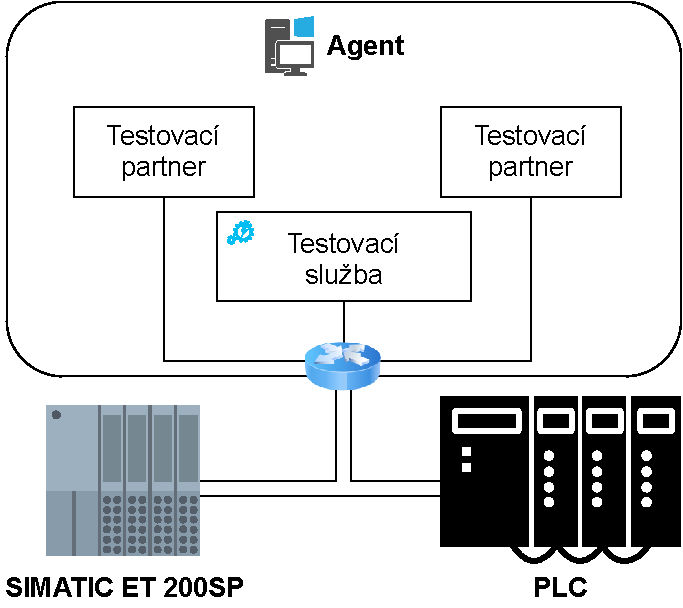
\includegraphics[width=0.97\textwidth]{assets/img/bp_assets/devicemodel.pdf}
    \caption{Ukázka možného propojení účastníků testování v původní knihovně}
    \source{Převzato z \cite{bakalarka}}
    \label{fig:bp_devicemodel}
\end{figure}


\subsection{Integrace do testovaného zařízení}

K tomu aby mohla být knihovna použita na zařízení, které je testováno, je zapotřebí nejdříve implementovat rozhraní pro testované zařízení. Implementací rozhraní jsou definovány primárně všechny potřebné funkce pro vytvoření spojení mezi testovaným zařízením a testovací službou. Zároveň definujeme funkci pro získávání instancí jednotlivých testů. 

Tyto testy rovněž dodržují jednotnou podobu pomocí rozhraní testu. Toto rozhraní definuje tři fáze testu:

\begin{enumerate}
    \item Příprava na testování -- definování potřebných struktur, inicializace.
    \item Testování -- provedení samotného testu.
    \item Úklid po testu -- uvolnění využitých zdrojů a uvedení zařízení do původního stavu.
\end{enumerate}

Všichni účastníci testu musí mít pro provedení daného testu obsahovat implementaci daného testu, definovanou rozhraním pro test, a musí být na základě obdržení identifikátoru testu schopni test instanciovat. To se provede registrací testu ve funkci \inlinecode{getTest}, která je definována rozhraním pro zařízení.

Testovací služba následně synchronizuje všechny účastníky, tak aby před započetím další testovací fáze všechna zařízení dokončila fázi předchozí. 

\subsection{Možnosti virtualizace v knihovně}

Původní testovací knihovna definuje již předem zmíněné testovací partnery, kteří jsou virtualizovaní participanti testů, sloužící k simulaci protistrany při testování průmyslové komunikace s testovaným zařízením. Jejich implementace kopíruje implementaci pro testované zařízení. Výhodou je, že k jejich využití je potřeba implementovat pouze samotné rozhraní pro test.

Každý testovací partner má životnost pouze v průběhu testu. To znamená, že před započetím testu je každý testovací partner vytvořen a připojen k testovací službě a následně po dokončení testu ukončen. Toto umožňuju variabilní počet testovacích partnerů pro každý testů.

\subsection{Topologie zapojení účastníků testu}

V případě verifikace průmyslové komunikace je samozřejmě podstatné, aby všichni účastníci testu byli schopni komunikovat mezi sebou dle potřeb daných testů. Aktuální knihovna ale toto nijak nekontroluje. 

Jediný požadavek knihovny je, aby každý účastník testu byl připojen k testovací službě a odpovídal na její požadavky. Samotné testované zařízení se připojuje před započetím testování a do konce všech testů připojeno. Testovací partneři, jak už jsem zmínil, se připojují dle potřeby před započetím jednotlivých testů.

Knihovna tedy nijak neřeší topologii zapojení jednotlivých zařízení. Je zde tedy předpoklad, že testovací partneři budou schopni komunikovat s ostatními účastníky testu díky tomu, že samotná testovací služba je schopna s nimi komunikovat. Zároveň, pokud by z nějakého důvodu komunikace nebyla možná, tak musí selhat samotné testy.

\subsection{Souhrn}

I když testovací knihovna přináší zjednodušení a automatizovaní testování průmyslové komunikace, tak stále je zde prostor pro zlepšení. Knihovna v aktuální podobě podporuje pouze limitovanou virtualizaci. Za pomoci knihovny jsme sice schopni simulovat protistranu, ale již ne samotné zařízení a to vždy musí běžet nezávisle na knihovně. 

Aktuální nový požadavek na řešení topologie zapojení zařízení nesplňuje vůbec. Zároveň je limitující požadavek, že pro každý test musí každý účastník testu obsahovat implementaci testu. Toto nemusí být vždy potřeba, například při testování veřejného rozhraní.

\section{Možnosti rozšíření virtualizačních prvků}

Z analýzy stávajícího stavu knihovny je vidět, že možnost virtualizace prostřednictvím stávající knihovny jsou limitované. Knihovna nepodporuje možnost simulovat jakékoliv zařízení a vůbec neřeší topologii zapojení daných zařízení. Rozšířením knihovny tedy chceme docílit větší možnosti virtualizace a simulace reálného prostředí. Nová knihovna by tedy měla cílit na

\begin{itemize}
    \item možnost spustit jakékoliv zařízení jako virtualizované,
    \item zapojit tato zařízení dle definované topologie (sériové linky, kruhu, hvězdy).
\end{itemize}


\subsection{Virtualizace zařízení}

Při virtualizaci zařízení máme na výběr více možností jak virtualizovat. První možnost je vytvoření virtuální mašiny pro každé zařízení prostřednictvím hypervizoru. Tato možnost sice splňuje podmínku na to spustit každé zařízení jako virtualizované, ale pro toto použití je nevhodné. 

Logickou možností je použití virtualizace skrz kontejnerizaci. Díky kontejnerizaci můžeme jednoduše spustit $n$ zařízení na jednom hardwaru. Pokud bychom měli virtuální mašiny pro $n$ zařízení, tak by zároveň muselo běžet $n$ operačních systémů, což snižuje efektivnost využití výpočetních zdrojů. Zároveň můžeme jednoduše a dynamicky vytvářet virtuální sítě, které budou splňovat požadovanou topologii. 

Toto potvrzují studie, které zkoumaly rozdíl ve výkonu a efektivnosti využití výpočetních zdrojů mezi kontejnerizací prostřednictvím softwaru Docker a virtualizačního řešení KVM, který umožnuje jádru fungovat jako hypervizor. Při jejich porovnání bylo zjištěno, že díky nástroji Docker jsou virtuální zařízení schopna být spuštěna rychleji a využívají méně výpočetních zdrojů. V porovnání při počítání HPC(High performance counting) úkolů, bylo dosaženo díky nástroji Docker lepšího výkonu o 42\,\% při úkolech náročných na procesor a o 14,98\,\% lepšího výkonu při úkolech náročných na interní paměť.\cite{kvmdockercomp}\cite{2021virt} \note{Asi bude potřebovat ještě uhladit v závuslosti na teoretické časti atd.}


\subsection{Porovnání kontejnerizačních řešení}

V dnešní době existuje mnoho řešení, který využívají kontejnerizaci. V následující sekci porovnám vybraná řešení a zhodnotím jejich vhodnost použití v testovací knihovně. 

K výběru je ale nejdříve potřeba nadefinovat úrovně správy, tedy oblasti, které můžou jednotlivé nástroje spravovat. Ty můžeme dle Aleksic\cite{docker_alt_23} rozdělit do čtyř kategorií:

\begin{description}
    \item[Image builders] Nástroje, které umožňují vytvářet kontejnery v souladu s pravidly dle OCI.
    \item[Container managers] V širším smyslu tak můžeme nazvat všechny nástroje, které pomáhají se sestavováním a během kontejnerů. Specificky ale tak můžeme nazvat ty nástroje, které pomáhají spravovat jednotlivé instance kontejnerů.
    \item[Container runtimes] Nástroje, které se starají o běh kontejnerů.
    \item[Container engines] Nástroje, které se starají o všechny procesy spojené s  kontejnerizací.
\end{description}

K úspěšnému využití kontejnerizace je samozřejmě potřeba spravovat všechny procesy spojené s kontejnerizací. Mým cílem je tedy primárně použít k řešení kontejnerizace tzv. \textit{container engines}. Jejich přímým využitím, oproti využití několika nástrojů, které by dohromady tvořili container engine, doufám předejití problémům s kompatibilitou a integrací těchto nástrojů dohromady.

Hlavním požadavkem na dané řešení je, aby podporovalo operační systém Windows. Tento požadavek primárně vyvstává z infrastruktury firmy Siemens. Vybranými řešeními tedy jsou

\begin{itemize}
    \item Docker,
    \item Podman,
    \item Vagrant. 
\end{itemize}


\subsection{Shrnutí}

Při pohledu na vytvořenou analýzu je vidět, že Vagrant vyšel z této analýzy na poslední příčce. Díky rozdílnému primárnímu zaměření pokulhává v několika kategoriích, především v efektivitě využití výpočetních zdrojů. Zároveň za tuto velkou cenu nepřináší žádné výhody oproti ostatním nástrojům.

Docker a Podman jsou velice podobné nástroje a ve spoustě případů je každý z nich dobrou volbou. Pro použití v testovací knihovně ovšem vyhrává Docker. Hlavním důvodem je jeho nativní podpora platformy Windows. Další velkou výhodou je jeho široká rozšířenost, což vede k velice aktivní komunitě vývojářů, jejichž knihovny a návody velice usnadňují jeho integraci. 

\chapter{Návrh}\label{chap:design}

V této kapitole se bude zabývat návrhem úprav a rozšíření původní testovací knihovny


\section{Souhrn požadavků}

K tomu abych mohl správně navrhnout úpravy v testovací knihovně, tak je dobré připomenout, co se od nové knihovny požaduje a proč. Knihovna by ve své nové podobě měla umět spouštět virtualizovaná zařízení a dle konfigurace vytvářet požadované topologie. Hlavní motivací je zvýšení flexibility knihovny, zvýšení možností využití a minimalizovaní zásahu do kódu testovaného zařízení, což vše vede ke snížení nákladů a úsilí na testování.  

Tyto kroky směřují k snížení závislosti na reálném hardwaru, na kterém daný produkt následně poběží. Hardware a primárně jeho architektura ve spoustě případů hraje důležitou roli. Jsou ovšem komponenty, jejichž chování je stejné, ať už poběží na jakémkoliv stroji. Jejich logika si nijak nemění. Přesunutím testů těchto komponent do virtualizovaného prostředí rozšíří možnosti, jak tyto komponenty testovat. Zároveň je možné mít mnohem více testovacích scénářů na různých topologiích. Je ale samozřejmé, že testy na reálném hardwaru budou vždy potřeba a nelze se této závislosti nijak zbavit.


\section{Návrh architektury}

Jednu z možných architekturu stávající testovací knihovny je možné vidět na obrázku \ref{fig:bp_devicemodel}. Jak lze vidět, testovací knihovna požadovala existenci alespoň jednoho fyzického zařízení, tedy reálného zařízení běžícího mimo zařízení, na kterém byla spouštěna testovací knihovna. 
Toto byla velice omezující podmínka, díky které nebylo možné virtualizovat samotné testované zařízení.

Představu nové architektury je možné vidět na obrázku \ref{fig:architecture}. Jak je na obrázku vidět, vše se již odehrává na tzv. agentovy, což je ve finále jakékoliv zařízení s potřebným softwarem pro virtualizaci. Všechna zařízení jsou přesunuta do virtualizovaného prostředí, které bude orchestrováno za pomoci softwaru Docker. 

Na obrázku lze vidět tři druhy zařízení, která jsou barevně oddělená. Zeleně označeným zařízením je původní \textit{testovací služba}. Ta řídí testovací běh a vyhodnocuje výsledky testů. Testovací služba běží přímo v operačním systému agenta, tedy bez žádné virtualizace. Uvnitř modře označeného virtualizovaného prostředí lze následně vidět jednu z možných simulovaných topologií, v tomto případě topologii hvězdy. 

Každý objekt uvnitř virtualizovaného prostředí představuje právě jedno zařízení, které je kontejnerizováno. \textit{Testované zařízení} představuje vyvíjený produkt, který chceme testovat. Ostatní oranžová zařízení představují \textit{testovací partnery} potřebné k testování. Rozdílem od stávající knihovny je, že ne všichni testovací partneři musí být k testovací službě připojeni. Na obrázku lze vidět, že v tomto případě pouze testovací partner 1 a 4 jsou připojeni k testovací službě. Je zde ale předpoklad, že alespoň jedno zařízení musí být k testovací službě připojeno.

Novým typem zařízení je červeně označený \textit{odposlouchávač komunikace}. Toto zařízení jak už z názvu vyplívá bude zaznamenávat komunikaci na právě jednom spojení dvou zařízení. Zároveň bude připojeno k testovací službě, což znamená že komunikace bude zaznamenávána pouze v průběhu testu a pro každý test bude vytvořen separátní záznam.

\begin{figure}[htbp]
    \centering 
    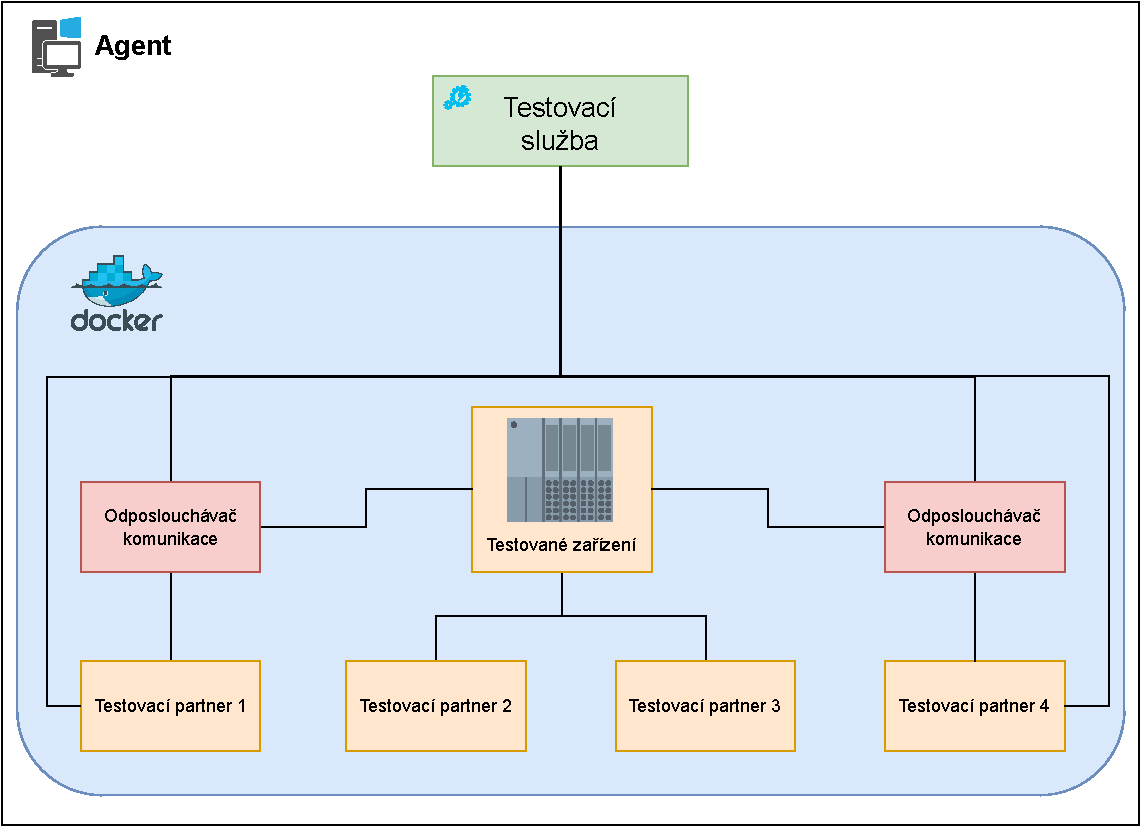
\includegraphics[width=\textwidth]{assets/img/architecture.pdf}
    \caption{Ukázka jedné z možných architektur nové testovací knihovny}
    \label{fig:architecture}
\end{figure}


\section{Orchestrace virtualizovaného prostředí}\label{sec:design_virt}

Důležitou součástí testovací knihovny bude implementace orchestrace virtualizovaného prostředí. To znamená, že testovací služba bude schopna vytvářet jednotlivá virtuální zařízení, které následně automaticky propojí dle požadované topologie a po konci testování daná zařízení ukončí. 

Knihovna bude obsahovat tři správce

\begin{enumerate}
    \item Správce kontejnerů, tedy zařízení
    \item Správce sítě
    \item Správce virtualizovaného prostředí
\end{enumerate}

Veškerá orchestrace bude procházet přes tyto správce. Správce virtualizovaného prostředí bude obsahovat oba předem zmíněné správce. Tyto budou mít na starost existenci daných zdrojů, dle názvu.

Virtualizované prostředí bude definované za pomoci konfiguračního souboru dle formátu YAML. Hlavní důvod proč využít YAML, místo původního formátu JSON, kterým bylo definováno nastavení testovací knihovny, je co nejbližší přiblížení se aktuálním konvencím v kontextu k Docker compose. Konfigurace bude tedy co nejvíce napodobovat jeho konfigurační soubor. 

První položkou v konfiguračním souboru bude položka \inlinecode{service}. Ta bude obsahovat pouze položku \inlinecode{connections}, která bude obsahovat počet zařízení, která se připojí k testovací službě. Toto číslo musí být větší než 0, jelikož testovací knihovna bude alespoň jedno zařízení vyžadovat.

Další položkou bude položka \inlinecode{containers}. Ta bude obsahovat informace o všech zařízeních, která v daném virtualizovaném prostředí budou. Klíčem každé položky uvnitř této sekce bude název zařízení, které bude fungovat pro referenci daného zařízení. Pro každé zařízení následně půjde definovat tato nastavení: 

\begin{description}
    \item[build] Definice zařízení, buď za pomoci obrazu (image) nebo cestou k docker souboru (Dockerfile). Toto bude označeno klíčem \inlinecode{image} a \inlinecode{dockerfile}, následovanou požadovanou hodnotou.
    \item[type] Typ zařízení, které bude vytvořeno. \customtodo{upřesnit}
    \item[cap\_add] Seznam \uv{schopností}, v tomto kontextu práv, které bude daný účet na kontejneru mít. Ty budou přidány ke právům, které v základu docker dává účtu vytvořenému v kontejneru. 
    \item[commands] Seznam příkazů, které budou spuštěny v kontejneru.
    \item[environment] Seznam proměnných, která budou v kontejneru nastaveny. Klíč bude název proměnné a jeho hodnota bude hodnotou proměnné
    \item[ports] Seznam mapování portů z kontejneru do prostředí hostitelského zařízení. Každý záznam obsahuje dva porty oddělené dvojtečkou, kdy první je port hostitelského zařízení a druhý je port kontejnerizovaného zařízení.
    \item[privileged] Boolean hodnota, zdali účet na kontejneru bude mít administrátorské práva.
    \item[logging] Boolean hodnota, která značí zdali je komunikace mezi tímto zařízením odposlouchávána. Tedy pokud je hodnota \inlinecode{true}, tak poté knihovna zařídí zaznamenávání všech spojů tohoto zařízení
    \item[tty] Boolean hodnota, která v původním docker compose značí připojení pseudo-terminálu ke kontejneru, který má za následek to, že kontejner po dokončení definovaných příkazů zůstane běžet. V kontextu knihovny bude znamenat to, že kontejner zůstane po dokončení všech příkazů definovaných v \inlinecode{commands} běžet. 
\end{description}

V neposlední řadě konfigurační soubor bude obsahovat položku \inlinecode{links}. Ta bude definovat jednotlivá propojení mezi zařízeními, tedy celkovou topologii. V tomto seznamu bude každá položka obsahovat názvy dvou zařízení oddělené dvojtečkou a pro každý záznam bude vytvořeno propojení mezi danými zařízeními.

Povinnou součástí konfiguračního souboru bude celá sekce \inlinecode{service}, sekce \inlinecode{containers}, kde musí být definována nejméně jedno zařízení, která musí obsahovat alespoň kolonky \inlinecode{build} a \inlinecode{type}, a sekce \inlinecode{links}. Ostatní budou nepovinné. Při existenci pouze jednoho zařízení může být testovací knihovna využita pro unit testy. 

Testovací knihovna bude kontrolovat, zdali testované prostředí bylo vytvořeno. Pokud ne, nezapočne testování. Zároveň bude kontrolovat zda všechna zařízení byla úspěšně spuštěna. Po konci testování testovací knihovna všechna zařízení ukončí, a vymaže všechny jím definované sítě, kontejnery atd.

Pro pohodlnost testovací knihovna bude také podporovat více různých topologií v rámci jednoho testovacího projektu. Při každé inicializaci virtualizovaného prostředí testovací služba porovná danou konfiguraci s aktuální konfigurací. Pokud budou konfigurace totožné, testovací služba ponechává prostředí nepozměněné, v opačném případě vyčistí virtualizované prostor, do kterého následně vloží nová zařízení a jejich nastavení.  


\section{Komunikace}

Komunikaci v rámci testovací knihovny lze rozdělit do dvou kategorií:

\begin{enumerate}
    \item komunikace mezi zařízeními,
    \item komunikace s testovací službou.
\end{enumerate}

Propojení mezi jednotlivými zařízeními bude zprostředkováno testovací knihovnou, respektive všechny zařízení budou propojena dle dané konfigurace, ale nebude nijak kontrolováno, pouze dle požadavku může být komunikace odposlouchávána a ukládaná. 

Komunikace s testovací službou bude probíhat za stejných podmínek, jako tomu je doposud. Testovací knihovna přesně definuje strukturu zpráv. Každá zpráva obsahuje v prvních dvou bajtech typ zprávy, v dalších dvou bajtech délku dat zprávy a případná data zprávy, jejichž délka je uložena v délce dat zprávy. Každá zpráva tedy musí mít minimálně 4 bajty. 

Možnou komunikaci mezi testovací službou a účastníky testu, tedy zařízeními uvnitř virtualizovaného prostředí, můžeme vidět na sekvenčním diagramu z mé bakalářské práce\cite{bakalarka}, který je na obrázku \ref{fig:seqdiag}. Na něm lze vidět, jak by probíhala komunikace při běhu o jednom testu. Jak jsem již ale zmínil dříve, nově ne všechna zařízení musí komunikovat s testovací službou. 

\begin{figure}[htbp]
    \centering 
    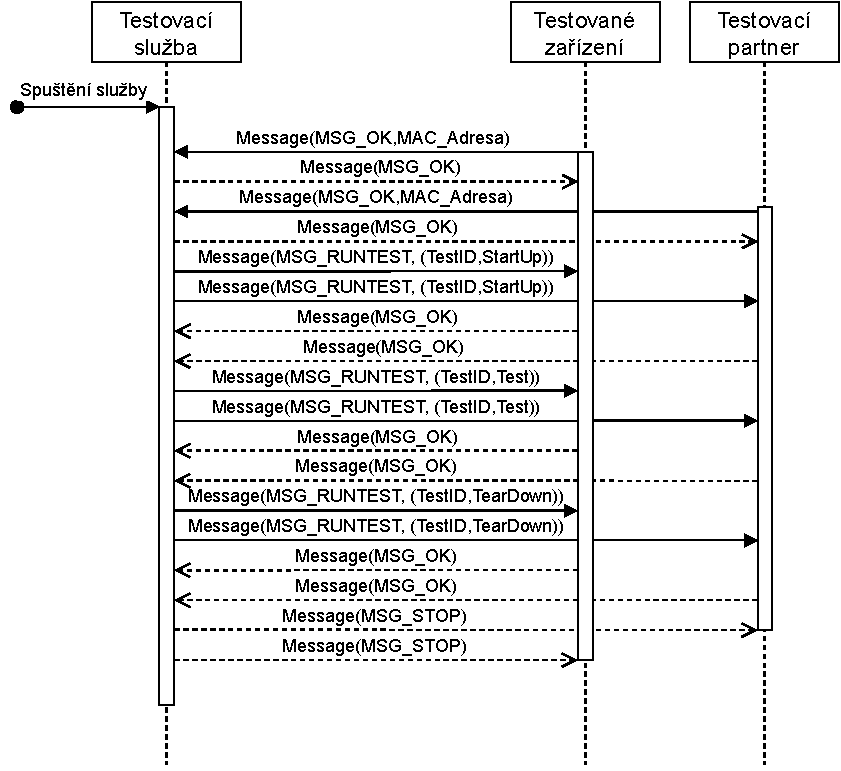
\includegraphics[width=\textwidth]{assets/img/bp_assets/sequencediagram.pdf}
    \caption{Sekvenční diagram ukázky komunikace mezi účastníky testování}
    \source{Převzato z \cite{bakalarka}}
    \label{fig:seqdiag}
\end{figure}

\section{Testovací služba}

Jádrem testovacího běhu zůstane testovací služba, která musí komunikovat a tím ovládat alespoň jedno zařízení. Ve stávající implementaci byla na počátku testování vytvořena jedna instance testovací služby, která existovala po celou dobu testování. Nově bude životnost testovací služba navázána na dané virtualizované prostředí. Tedy, testovací služba vznikne až po úspěšném vytvoření virtualizovaného prostředí. Při změně virtualizovaného prostředí bude testovací služba ukončena a po vytvoření nového prostředí spuštěna nová instance.

Fungování testovací služby lze vidět na novém diagramu aktivit testovací služby na obrázku \ref{fig:activitydiagramservice}, na kterém jsou označeny i změny oproti původnímu diagramu aktivit testovací služby.

\begin{figure}[htbp]
    \centering 
    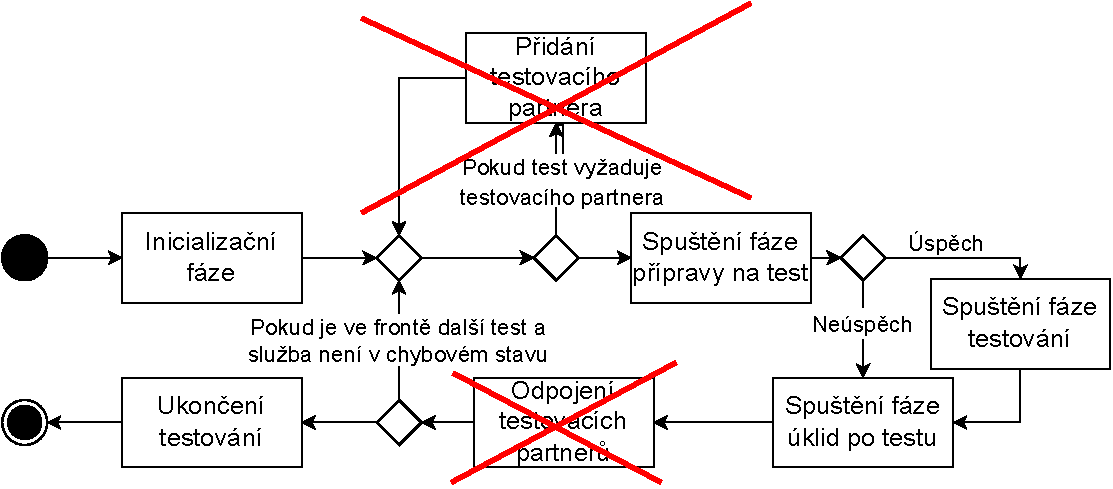
\includegraphics[width=\textwidth]{assets/img/activitydiagramservicechange.pdf}
    \caption{Nový diagram aktivit testovací služby}
    \source{Vytvořeno dle předlohy z \cite{bakalarka}}
    \label{fig:activitydiagramservice}
\end{figure}

Po sestavení virtualizovaného prostředí testovací služba započne inicializační fázi, ve které se všechna zařízení ovládaná testovací službou připojí k testovací službě. Tedy mimo přímých účastníků testu se v této fázi připojí i všichni odposlouchávači komunikace, pokud nějací existují. 

Testovací služba sama o sobě nemá ponětí o tom, které testy budou spuštěny a které ne, ale pouze zpracovává požadavky, které na ni přichází. Tedy po obdržení požadavku na spuštění testu testovací služba spouští všechny fáze testu. Při ukončení testovací služba odesílá všem připojeným účastníkům zprávu o ukončení testování, čímž mohou být připojená zařízení taktéž ukončena. O úspěšné ukončení se ovšem stará integrace virtualizovaného prostředí.

\section{Testování}

Nová testovací knihovna zachová proces testování a podobu jednotlivých testu ve stejné podobě jako tomu bylo doposud. K tomu aby bylo možné testovat za použití testovací knihovny, tak je potřeba implementovat rozhraní pro testované zařízení, které definuje potřebné funkce ke komunikaci s testovací službou. 

Definované rozhraní je ale v rámci terminologie nyní lepší nazvat jako rozhraní pro účastníka testu, jelikož rozhraní může využít jakékoliv zařízení, které je potřeba synchronizovat s testovací službou. I v aktuální implementaci testovací partneři obsahovali implementaci tohoto rozhrání a jejich běh byl identický. 

Pro připomenutí, rozhraní pro test následně definuje tři fáze testu, které jsou:

\begin{enumerate}
    \item Příprava na testování -- definování potřebných struktur, inicializace.
    \item Testování -- provedení samotného testu.
    \item Úklid po testu -- uvolnění využitých zdrojů a uvedení zařízení do původního stavu.
\end{enumerate}

Běh účastníka testu, který je připojen k testovací službě, můžeme vidět na diagramu aktivit na obrázku \ref{fig:act_diag_device}. Jeho aktivity zůstanou identické. Změna nastává v definovaných synchronizačních bodech, které jsou na obrázku označeny modře. 

Testovací služba obdrží informace o dokončení každé fáze testu pouze od těch účastníků, co jsou k ní připojený. Tedy, pokud je potřeba synchronizovat nějaké zařízení, které není připojeno k testovací službě, tak potom by toto byl úkol jednoho z testovacích partnerů, který k testovací službě připojen je. Zároveň zde existuje možnost vytvořit testovacího partnera, který pouze kontrolovat správnost daného zařízení. 

\begin{figure}
    \centering 
    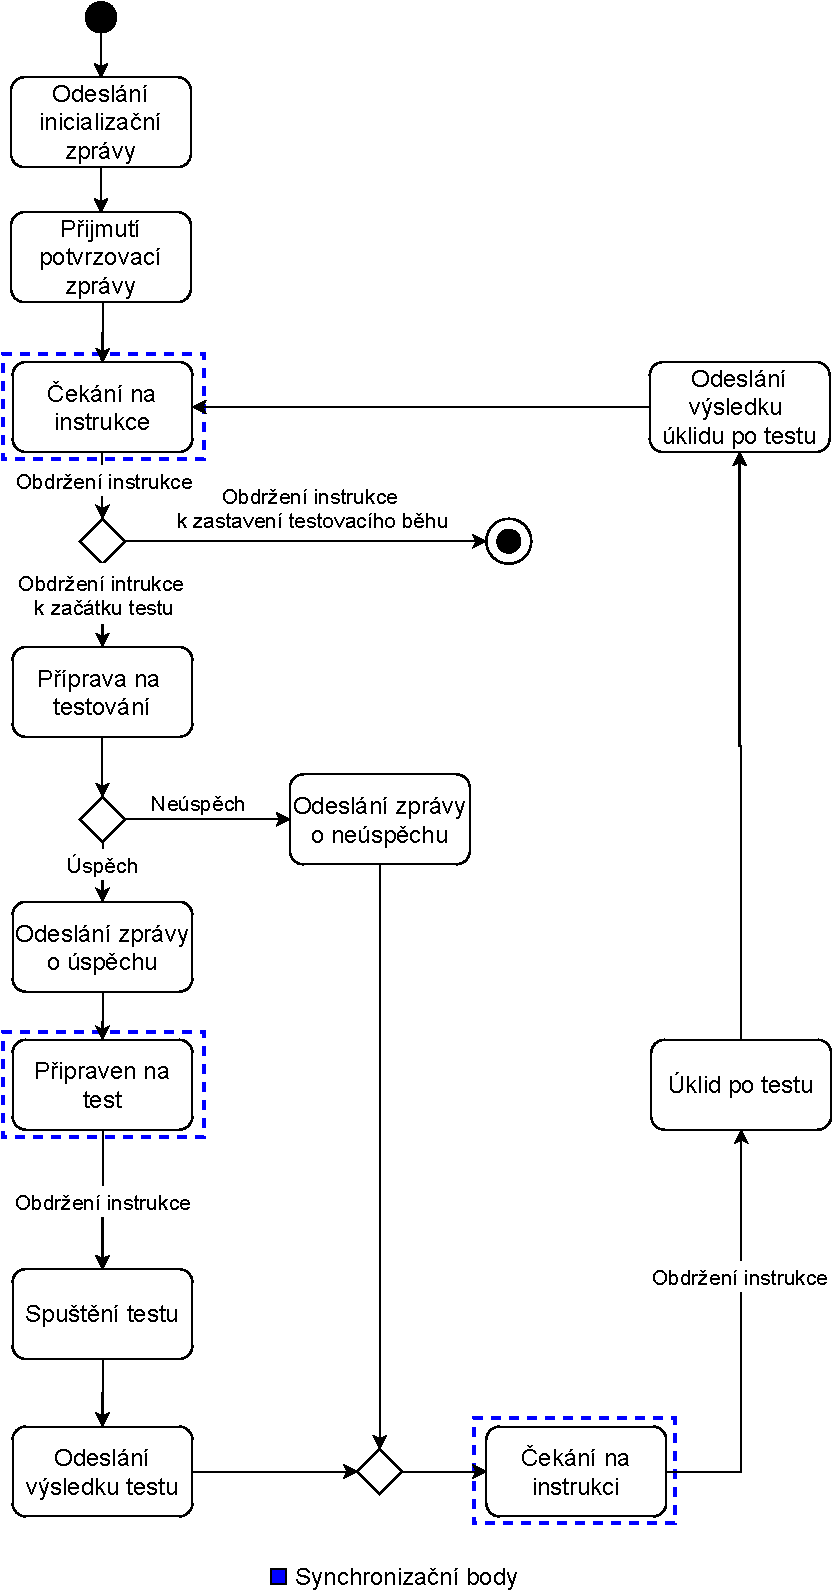
\includegraphics[height=0.98\textheight]{assets/img/bp_assets/activitydiagramdevice.pdf}
    \caption{Diagram aktivit účastníka testu}
    \label{fig:act_diag_device}
\end{figure}





\chapter{Implementace}\label{chap:implementation}

V této kapitole se budu věnovat implementaci navržených úprav z kapitoly \ref{chap:design}.


\section{Příprava stávající implementace testovací knihovny}
Původní testovací knihovna obsahovala toto rozdělení implementace, dle zdrojových složek:

\begin{itemize}
    \item \inlinecode{core} - implementace celé testovací knihovny v jazyce \csharp, tedy implementace testovací služby, testovacích partnerů atd.
    \item \inlinecode{cpp} - implementace pro účastníka testování v jazyce \cpp, včetně potřebných rozhraní.
\end{itemize}

V předchozí implementaci nebylo potřeba žádné zařízení vytvářet externě mimo testovací projekt. Proto veškerá implementace v jazyku \csharp\, byla v jednom celku. Ovšem účastník testu vůbec nepotřebuje implementaci testovací služby a integraci virtualizovaného prostředí. Proto tedy bylo logické rozdělit testovací knihovnu na tyto logické celky:

\begin{itemize}
    \item \inlinecode{TestLib.Core} (složka \inlinecode{core}) - jádro testovací knihovny, které obsahuje všechna potřebná rozhraní, definice zpráv a správce běhu testovacího partnera, respektive účastníka testu.
    \item \inlinecode{TestLib} (složka \inlinecode{test\_lib}) - celá testovací knihovna, která mimo jádra testovací služby obsahuje testovací službu, integraci virtualizovaného prostředí a další pomocné entity. Jádro testovací knihovny je přidáno jako závislost. 
\end{itemize}

S využitím \inlinecode{TestLib.Core} je tedy uživatel se připojit k testovací službě, která následně může ovládat testovací běh na zařízení. Tato implementace je skoro identická s implementací v jazyce \cpp. Nově zde přibyla i implementace v jazyce Python. Ta vznikla z důvodu pohodlnosti testerů, kteří mají velikou část testů napsanou právě v tomto jazyce. Pomoci ní budou schopni jednodušeji integrovat stávající testy do nové testovací knihovny. 


\section{Orchestrace virtualizovaného prostředí}
Testovací knihovna k úspěšnému vytvoření potřebuje primárně umět tyto aktivity:

\begin{enumerate}
    \item Umět komunikovat se softwarem Docker.
    \item Vytvořit kontejnery, tedy virtualizované zařízení, dle konfigurace.
    \item Propojit všechna zařízení mezi sebou taktéž dle konfigurace.
\end{enumerate}

\subsection{Komunikace se softwarem Docker}
Orchestrace virtualizovaného prostředí má dle návrhu probíhat s pomocí softwaru Docker. 
Jako první tedy bylo potřebovat integrovat komunikaci se softwarem Docker do testovací knihovny. Před vytvořením vlastní integrace jsem se ovšem jako první porozhlédnul po dostupných komunitních knihovnách, které už toto připojení integrují, zda nějaká z nich není vhodná pro použití v testovací knihovně. 

Testovací knihovna je sepsána v jazyce \csharp, proto jsem tedy primárně vyhledával za pomoci softwaru NuGet\cite{nuget}, který slouží jako správce balíčků, tedy externích knihoven, v jazyce \csharp\, a ekosystému .NET. Z dostupných knihoven mě primárně zaujali dvě - Docker.Dotnet\cite{dockerdotnet} a Fluent.Docker\cite{fluentdocker}. 

Docker.Dotnet je open-source knihovna vytvořená a spravovaná .NET Foundation. Tato nezisková organizace, založena společností Microsoft, se stará o zlepšování open-source ekosystému okolo .NET platformy\cite{dotnetfoundation}. Lze ji tedy v podstatě označit jako \uv{oficiální} integraci softwaru Docker do .NET ekosystému, i když fakticky je komunitním dílem. 

Oproti tomu knihovna Fluent.Docker je open-source knihovna původně od vývojáře Mario Toffia, na které se ale dnes podílelo nějakým dílem již 30 vývojářů. Knihovna se primárně zaměřuje na integraci tzv. Fluent rozhraní, které dovoluje řetězit metody za sebou, díky tomu, že každá metoda vrací instanci třídy, ze které je metoda volaná. \cite{fluentinterface}

Obě knihovny jsou ve spoustě aspektech srovnatelné - obě jsou open-source knihovny vytvořené komunitou a obě jsou vhodné pro komerční použití. K integraci jsem ovšem zvolil knihovna Fluent.Docker. Tato knihovna obsahuje větší abstrakci jednotlivých příkazů a je tedy mnohem jednoduší na použití a integraci.

\subsection{Správa sítě}

Správu virtualizované sítě má v nové knihovně na starost třída \inlinecode{NetworkManager}, která se stará o vytváření, nastavení a nakonec i destrukci sítě. 
Samotná realizace vytváření a destrukce sítí v prostředí softwaru Docker je ovšem realizována prostřednictvím třídy \inlinecode{DockerNetworkDriver}. Tato třída obsahuje metodu \inlinecode{CreateNetwork(string, int)}, kde jako argumenty požaduje název sítě a počet dostupných IP adres. Toto číslo ovšem musí zahrnovat i počet implicitně obsazených IP adres - tedy IP adresu sítě, broadcast adresu a pro Docker i IP adresu směrovače. Informace o počtu potřebných implicitních zařízeních je uložena ve statické třídě \inlinecode{NetworkConstants}.

Metoda \inlinecode{CreateNetwork} nejdříve zjistí, jaké rozsahy IP adres jsou obsazené a jaké rozsahy jsou volné. Následně na základě těchto informací vytvoří nejmenší možnou síť, do které se bude vejít požadovaný počet IP adres. Zároveň třída se snaží  co nejvíce vyplňovat mezery mezi adresními prostory. Metoda následně pouze vrací instanci třídy \inlinecode{NetworkInfo}, která obsahuje všechny potřebné informace o dané síti. Třída \inlinecode{DockerNetworkDriver} si udržuje instance všech vytvořených sítí, aby byla schopna následně při ukončování vytvořené sítě smazat. 

Třída \inlinecode{NetworkManager} má k vytvoření sítě tyto tři metody:

\begin{enumerate}
    \item \inlinecode{AddNode(string)} - přidání zařízení (kontejneru) do správce, kde argumentem je identifikátor zařízení
    \item \inlinecode{AddConnection(string, string)} - přidání propojení mezi dvěma zařízeními, kde argumentem jsou identifikátory zařízení, mezi kterýma má býti spojení
    \item \inlinecode{BuildNetwork()} - metoda, která spustí výpočet a následné vytvoření sítě ve virtualizovaném prostředí
\end{enumerate}

Pro vytvoření úspěšného propojení mezi dvěma zařízeními je potřeba přidat všechna zařízení za pomoci funkce \inlinecode{AddNode}, jinak třída vyhodí výjimku při sestavování sítě. Po zaregistrovaní všech zařízení a všech propojení je zavolána metoda \inlinecode{BuildNetwork}. 

Tato metoda nejdříve vytvoří strukturu uložení všech informací o síti a kontejnerech. Metody \inlinecode{AddNode} a \inlinecode{AddConnection} totiž pouze přidají dané informace do front, které jsou v tento moment zpracovávány za pomoci metody \inlinecode{ConstructDataStructure}. Metoda nejdříve pomocí metody \inlinecode{RegisterNode} zaregistruje všechny zařízení, což vede hlavně k přirazení unikátního indexu všem zařízením. Reference mezi jménem a indexem je uložena ve slovníku \inlinecode{nodeMapper}. 

Následně metoda zaregistruje s pomocí metody \inlinecode{RegisterConnection} všechna spojení, což znamená že dvojice indexů zařízení, mezi kterýma má existovat spojení, jsou přidány do seřazené množiny, která je uložena v atributu \inlinecode{connections}. Tyto dva indexy jsou ovšem v relaci a platí $\forall x,y \in K, xSy \Rightarrow ySx$, kde $K$ představuje množinu všech indexů zařízení a $S$ je binární relace spojení zařízení zařízení.
Proto do atributu \inlinecode{connections} jsou ukládány obě symetrické hodnoty, primárně pro zjednodušení vyhledávání v této kolekci.

Jednotlivé informace o síťovém nastavení zařízení jsou uložena v seznamu \inlinecode{nodeConfigurations}, který je indexován za pomoci atributu \inlinecode{nodeMapper}. Ten obsahuje instance třídy \inlinecode{ContainerNetworkConf}, která obsahuje informace o všech sítích, ke kterým je dané zařízení připojeno a jakou má v něm přiřazenou IP adresu, o adrese implicitního směrovače a seznam všech statických směrování. Statická směrování jsou reprezentována za pomoci třídy \inlinecode{NetworkRoute}, jehož instance obsahuje všechny potřebné informace. 

Samotné reálné vytváření sítě počíná vytvořením tzv. správcovské sítě, do které budou připojena všechna zařízení. Ta slouží primárně pro případnou komunikaci s testovací službou. Tato síť je typu bridge. Všechna zařízení budou mít nastavena směrovač této sítě jako implicitní bránu.

Následně třída pro každé spojení vytvoří separátní síť typu bridge. Na první pohled se může zdát, že toto je velice neefektivní řešení. Důvod, proč jsem zvolil toto řešení, je ovšem kvůli technologickému omezení. V každé síti typu bridge je vytvořen implicitní směrovač, který rozesílá komunikaci daným kontejnerům. Tím pádem, každá komunikace v základním nastavení jde z odchozího kontejneru do směrovače a následně do cílového kontejneru. Tím by ale byla porušena požadovaná topologie. Z tohoto důvodu je pro každý spoj vytvořena nová síť. Za pomoci statického směrování je pak následně možné směrovat komunikaci do každého zařízení dle požadované topologie. 

Metoda tedy nejdříve vytvoří s pomocí metody \inlinecode{CreateNetwork} pro každé připojení síť a informace o dané síti uloží seznamu \inlinecode{networkInfos}. Index sítě je následně uložen do slovníku \inlinecode{networkIndexer}, kde klíčem je dvojice indexů zařízení, mezi kterýma daná síť, a tedy spojení, existuje. Oproti atributu \inlinecode{connections}, slovník neobsahuje obě symetrické hodnoty indexů. Platí, že $\forall x \forall y; x,y\in K; (x,y) \in \inlinecode{networkIndexer.Keys} \Rightarrow x < y$. 

Po vytvoření všech sítí metoda vypočítá statického směrovaní pro každé zařízení. Tento proces si zaslouží přiblížení. Metoda iteruje pro všechny zařízení všechny položky ve slovníku \inlinecode{networkIndexer}. Pokud mezi zařízeními existuje přímé spojení tak směrování je jednoduché, daná síť je směrována na dané přilehlé zařízení. Problem nastává, pokud síť není přímo připojena k zařízení. V tento moment je potřeba zjistit, jakým \uv{směrem} má být zpráva odeslána pro úspěšné doručení.

Nejbližší cesta do dané sítě je zjišťována za pomoci algoritmu BFS, jenž je implementován ve stejnojmenné metodě. BFS, neboli Breadth first search, funguje na principu prohledávání do šířky. Algoritmus nejdříve obdrží informace o počátečním a konečném zařízení, tedy o uzlech, mezi kterými má nalézt cestu. 

V počátku si algoritmus vytvoří frontu uzlů ke zpracování a seznam navštívených uzlů. Následně do fronty je vložen počáteční uzel a označen jako navštívený. Algoritmus následně ve smyčce skrz všechny položky fronty zkoumá jednotlivé uzly. Po vyjmutí prvního uzlu z fronty algoritmus zkoumá všechny jeho sousední uzly. Pokud sousední uzel ještě nebyl navštíven, tak poté je přidán na konec fronty. Po prozkoumání všech sousedních uzlů algoritmus pokračuje na další položku ve frontě. Součástí jednotlivých položek ve frontě je mimo informace o uzlu, který má být zpracován, také seznam uzlů, který reprezentuje cestu do daného uzlu k zpracování z počátečního uzlu. V případě, kdy uzel, který má být zpracován, je shodný s koncovým uzlem, tak je navrácen seznam uzlů reprezentující cestu do koncového uzlu. Pokud není nalezena cesta, tak poté metoda navrací prázdný seznam.

Pomocí tohoto algoritmu je tedy zjištěna nejkratší cesta do dané sítě. Tato cesta je nalezena v nejhorším případě v komplexitě $O(|V| + |E|)$, kde $|V|$ je počet uzlů, neboli kontejnerizovaných zařízení, a $|E|$ je počet hran mezi uzly, neboli spojení mezi zařízeními. Zároveň metoda pro každé zařízení může být volána maximálně $|V| - 1$ krát. Tyto vlastnosti jsou naprosto dostačující pro aktuální použití.\customtodo{Citovat bfs}

Metoda tedy navrací seznam zařízení, bez počátečního zařízení, který reprezentuje cestu od počátečního zařízení do cílového zařízení, neboli do dané sítě. Podstatnou informací je první položka v seznamu, tedy to sousední zařízení, kterému musí být zpráva odeslaná z daného zařízení, aby dosáhla cílového. To je nastaveno jako směr, kterým mají být všechny zprávy do dané sítě odesílány. Tímto způsobem implementace je testovací knihovna schopna nastavit všechny požadované topologie. Zároveň vždy odesílá zprávy nejkratší možnou cestou.

\subsection{Správa kontejnerů}\label{sec:cont_managment}

Stejně jako síť, i kontejnery mají svého správce, realizovaného třídou \inlinecode{ContainerManager}. Každý kontejner je podobně jako v případě sítí registrován s pomocí metody \inlinecode{AddContainer(string, ContainerConf)}, kde metoda obdrží v argumentech název a nastavení zařízení, získaného z konfiguračního souboru. To je uloženo do fronty pro následné zpracování.

Po přidání všech zařízení je možné zavolat metodu \inlinecode{Build}. Ta očekává jako argument instanci třídy \inlinecode{NetworkManager}, která již má vypočítané nastavení sítě daných zařízení. Nastavení pro jednotlivé zařízení jsou získávána za pomoci metody \inlinecode{NetworkManager.GetContainerConf(string)}, kde argumentem je název zařízení. 

Metoda \inlinecode{Build} následně zpracovává všechna zařízení ve frontě. Pokud obraz na zařízení je definován za pomoci Dockerfile, tak poté před vytvořením zařízení metoda \inlinecode{BuildImage} sestaví daný obraz. Metoda nejdříve zkontroluje, zdali daný obraz Dockerfilu již nevytvořila. Tuto kontrolu provádí tím, že při vytvoření si uloží hash zdrojového souboru do slovníku \inlinecode{imageTags}, kde hash souboru je klíčem a následně název vytvořeného obrazu je hodnotou ve slovníku. Po zajištění existence obrazu tedy metoda \inlinecode{BuildImage} vrátí název odpovídajícího obrazu. 

Vytvoření samotného kontejneru je následně provedeno metodou \inlinecode{CreateContainer}. Ta dostane jako argument název zařízení, název obrazu, instanci nastavení zařízení a instanci nastavení sítě zařízení. 

Každá kontejner je definovaný za pomoci rozraní \inlinecode{IVMContainer}, definovaného v sekci \label{sec:cont_design}. Pomocí jeho metod je každý kontejner nastavován a realizace těchto nastavení je poté na dané implementaci rozhraní. V aktuální implementaci existují tyto dvě implementace kontejnerů: 

\begin{itemize}
    \item \inlinecode{DefaultContainer} - základní kontejner vycházející z operačního systému Ubuntu. Reprezentován je enumerátorem \inlinecode{ContainerType.DEFAULT} 
    \item \inlinecode{NetworkLogger} - kontejner, který zajišťuje odposlouchávání sítě. Reprezentován je enumerátorem \inlinecode{ContainerType.NETWORK\_LOGGER}
\end{itemize}

Oba dva typy kontejnerů jsou rozlišeny za pomoci enumerátoru \inlinecode{ContainerType}. Každá jeho hodnota by měla být napsána velkými písmeny. V konfiguračním souboru se následně preferuje verze s malými písmeny, i když jakákoliv kombinace velkých a malých písmen bude akceptována. 

Následně rozšiřující statická metoda enumerátoru \inlinecode{GetInstance} dokáže vytvořit instanci daného typu kontejneru. Metoda zároveň obdrží argumenty pro konstruktor daného kontejneru. Hlavními argumenty jsou název kontejneru a název obrazu kontejneru. Kontejner typu \inlinecode{NetworkLogger} může ještě obdržet instanci třídy \inlinecode{ServiceConfiguration}, díky které obdrží nastavení testovací služby, ke které se následně připojí. 

Metoda \inlinecode{CreateContainer} následně vrátí instanci kontejneru, která je následně uložena do slovníku \inlinecode{containers}, kde klíčem je název zařízení. 

\subsection{Správce celého virtualizovaného prostředí}

Předchozí zmíněné správce je potřebo orchestrovat společně. K tomuto slouží třída \inlinecode{VirtualEnvironmentManager}. Třída obdrží instanci \inlinecode{EnvironmentConfiguration}, která reprezentuje nastavení virtualizovaného prostředí definovaného v sekci \ref{sec:design_virt}. Následně také obdrží instanci třídy \inlinecode{ServiceConfiguration}, ve které je obsaženo nastavení testovací služby.

Třída v sobě obsahuje instance obou dvou správců \inlinecode{NetworkManager} a \inlinecode{ContainerManager}. V konstruktoru je zavolána metoda \inlinecode{SetupEnvironment}, která zaregistruje všechny zařízení a připojení mezi nimi. Zároveň, pokud dle nastavení je potřeba zachytávat na daném spojení komunikaci, tak také přidá adekvátně dané odposlouchávače komunikace. 

Zavoláním metody \inlinecode{Build} je následně vytvořeno celé prostředí. Nejdříve je vytvořena požadovaná síť a následně jsou vytvořeny všechny kontejnery. Na konci metoda spustí všechny kontejnery.

Za pomoci metody \inlinecode{Stop} je poté následně možné zastavit všechny kontejnery. Nakonec, metodou \inlinecode{Dispose} jsou následně odstraněny všechny vytvořené prostředky prostřednictvím daných správců. 

\subsection{Ošetření chyb}

Implementace virtualizovaného prostředí ošetřuje všechny chyby tím, že v případě jejich vzniku vyhodí odpovídající výjimku. Je tedy potřeba následně tyto chyby v případě jejich vzniku zachytávat a adekvátně vyhodnotit.

Ovšem, pokud je program násilně ukončen, tak může dojít k nesmazaní daných vytvořených prostředků v Docker prostředí. To může způsobit jejich akumulaci a v případě sítě dokonce selhání vytvoření sítě. Testovací knihovna proto definuje ve statické třídě \inlinecode{TestLibConstants} proměnnou \inlinecode{ResourcePrefix}, který je přidán ke všem vytvořeným prostředkům.

Díky tomu může knihovna identifikovat jím vytvořené prostředky. Každý správce má tedy implementovanou metodu pro odstranění zbylých prostředků. Ty jsou volány prostřednictvím metody \inlinecode{RemoveHangingResources} v konstruktoru správce virtualizovaného prostředí před započetím všech akcí k vytvoření nového prostředí.

\subsection{Definice kontejnerů}

Jak jsem již řekl v sekci \ref{sec:cont_managment}, tak aktuálně testovací knihovna definuje dvě zařízení. Zařízení typu \inlinecode{default} je výchozím zařízením pro všechny aktuální kontejnery. Zařízení vychází z operačního systému Ubuntu 22.04\customtodo{citovat}. 

K správné orchestraci zařízení potřebuje kontejnerizované zařízení obsahovat potřebné nástroje k nastavení sítě. Všechny tyto nástroje jsou definované v novém obraze názvaném \inlinecode{testlib-ubuntu-base}. Tím pádem všechny kontejnery, které budou vycházet z tohoto obrazu, bude možné použít v testovací knihovně. 

Tento obraz následně může být distribuován, ať už do veřejného, nebo soukromého repositáře. Označení verze obrazu bude kopírovat označení podkladového obrazu operačního systému Ubuntu. Tedy, verze bude stejná, jako verze operačního systému Ubuntu. 

\subsection{Odposlouchávání komunikace}

K odposlouchávání komunikace byl vytvořen nový program pod názvem \inlinecode{NetworkLogger}. Program využívá knihovnu SharpPcap\cite{sharppcap} pro zachytávání komunikace na daném virtuálním rozhraní. 

Program přijímá variabilní počet argumentů v závislosti na módu fungování. Program podporuje dva módy fungování

\begin{enumerate}
    \item Mód bez připojení k testovací službě
    \item Mód s připojením k testovací službě
\end{enumerate}

K aktivaci prvního módu je potřeba předat programu přepínač \inlinecode{--no-service}, který mód aktivuje. Následně program očekává seznam názvů rozhraní, oddělených mezerou, ze kterých má zachytávat komunikaci. Při spuštění program zachytává všechnu komunikaci na daných rozhraní a následně vypisuje jednotlivé zachycené zprávy na standardní výstup.

V druhém módu testovací knihovna očekává tyto poziční argumenty:

\begin{enumerate}
    \item Složku, kde bude ukládat zachycené zprávy do souboru.
    \item Adresu, na které běží testovací služba.
    \item Port, na kterém běží testovací služba.
    \item Variabilní počet jmen rozhraní, které má zaznamenávat, oddělený mezerou.
\end{enumerate}

Po obdržení těchto argumentů se program připojí k testovací službě a projde stejnou inicializační fází, jako všichni ostatní účastníci testu. Následně po obdržení zprávy o započnutí testu započnuto zaznamenávání sítě. Symetricky, zaznamenávání sítě je ukončeno při obdržení zprávy o ukončení testu. Jednotlivé testy jsou tedy zaznamenávány separátně a pro každý test je vytvořen separátní záznam, rozlišen identifikátorem testu.

Program má definovaný Dockerfile, vycházející z definovaného obrazu \inlinecode{testlib-ubuntu-base}, na základě něhož může být program spuštěn ve virtualizovaném prostředí prostřednictvím softwaru Docker. To je přímo podporováno od Visual Studia 2022\cite{vs2022}, ve kterém jsou všechny projekty tvořeny. Při otevření projektu je vytvořen Docker kontejner, ve kterém se dá projekt následně spouštět a i ladit.

Za pomocí Visual Studia 2022 lze také uveřejnit daný program do Docker repositáře. Po vybrání \inlinecode{Publish} je možné program zveřejnit buď do veřejného Docker repositáře, nebo do soukromě hostovaného repositáře.

Zveřejněný program, neboli obraz, v základu spouští program v módu bez připojení k testovací službě. To lze při vytváření kontejneru změnit a tedy program správně nastavit. 

\section{Úprava testovací služby}

\note{Některé věci je ještě potřeba dodělat, aby to bylo konzistentní, dopíšu potom}

\section{Integrace virtualizovaného prostředí do testovací knihovny}

Pro integraci virtualizovaného prostředí je potřeba integrovat virtualizované prostředí do služeb testovací knihovny. Původní třída \inlinecode{ServiceRunner} byla přejmenovaná na \inlinecode{ServicesRunner}, aby název lépe reflektoval její zónu odpovědnosti. Ta v sobě obsahuje instance tříd \inlinecode{TestService} a \inlinecode{VirtualEnvironmentManager}.

Do statické třídy \inlinecode{API} byla přidána statická metoda \inlinecode{BuildEnvironment}. Tato metoda obdrží v argumentu cestu ke konfiguračnímu souboru daného virtualizovaného prostředí. Metoda načte danou konfiguraci a následně zavolá metodu \inlinecode{ServiceRunner.StartServices(EnvironmentConfiguration)}. Za pomoci ní je vytvořeno dané virtualizované prostředí. Nejdříve je ovšem zkontrolováno, zdali dané prostředí již není vytvořeno. Pokud ano, metoda ponechává dříve vytvořené prostředí. V opačném případě metoda ukončí testovací službu a zničí předchozí virtualizované prostředí (pokud nějaké existuje). Následně na to vytvoří nové virtualizované prostředí. Po úspěšném vytvoření prostředí je následně spuštěna testovací služba.

Použití této funkce je zamýšleno v rámci jednotlivých tříd testů. Testovací knihovna používá knihovnu MSTest pro propojení se serverem Azure DevOps, který může automaticky spouštět jednotlivé testy. Všechny testy musí být shlukovány do jednotlivých testovacích tříd. Testovací knihovna MSTest definuje atribut \inlinecode{ClassInitialize}. Metoda s tímto atributem bude spouštěna právě jednou před započetím testů v dané třídě. Je tedy logické shlukovat jednotlivé testy dle konfigurace virtualizovaného prostředí. Tímto použitím se minimalizuje riziko zbytečného přestavování virtualizovaného prostředí. 

Třída \inlinecode{API} také nově definuje metodu \inlinecode{SetServiceConfig}, díky které může být změněno základní nastavení testovací služby. 




% \chapter{Demonstrace použití knihovny}\label{chap:demonstration}


% \chapter{Vyhodnocení vytvořeného řešení}\label{chap:evaluation}


\begin{conclusion}

\end{conclusion}


{
    \setlength{\emergencystretch}{3em} 
    \def\UrlBreaks{\do\/\do\-\do\_}
    \printbibliography
}

\appendix

\chapter{Seznam použitých zkratek}
\begin{description}
	%\item[ADU] Application Data Unit
	\item[API] Application Programming Interface
	\item[BFS] Breadth First Search 
	%\item[CIP] Common Industrial Protocol
	%\item[EtherNet/IP] EtherNet Industrial Protocol
	\item[I/O] Input/Output
	\item[IDE] Integrated Development Environment 
	\item[ISA] Instruction Set Architecture 
	%\item[IP] Internet Protocol 
	\item[JSON] JavaScript Object Notation
	\item[HAL] Hardware Abstraction Layer
	\item[HPC] High performance counting
	\item[MB/s] Megabyte za sekundu
	\item[OCI] Open Container Initiative
	\item[OS] Operační systém 
	%\item[PDU] Protocol Data Unit 
	\item[PLC] Programmable Logic Controller
	\item[QA] Quality assessment 
	\item[REST] Representational State Transfer
	%\item[TCP/IP] Transmission Control Protocol/Internet Protocol 
	%\item[XML] Extensible markup language
	\item[VM] Virtual machine
	\item[YAML] YAML Ain't Markup Language
\end{description}

\chapter{Obsah přílohy}

\begin{figure}
	\dirtree{%
		.1 README.txt\DTcomment{stručný popis obsahu SD karty}.
		.1 impl\DTcomment{zdrojové kódy implementace}.
        .2 base\_docker\_image\DTcomment{výchozí Docker obraz}.
        .2 core\DTcomment{implementace jádra testovací knihovny v jazyku \csharp{}}.
        .2 cpp\DTcomment{implementace jádra testovací knihovny v jazyku \cpp{}}.
        .2 python\DTcomment{implementace jádra testovací knihovny v jazyku Python}.
        .2 test\_lib\DTcomment{implementace testovací knihovny v jazyku \csharp{}}.
        .2 test\_project\DTcomment{testovací projekt vytvořený k demonstraci funkčnosti}.
		.1 package\DTcomment{adresář se zkompilovanými NuGet balíčky testovací knihovny}.
		.1 text\DTcomment{text práce}.
        .2 src\DTcomment{zdrojová forma práce ve formátu \LaTeX{}}.
        .2 thesis.pdf\DTcomment{text práce ve formátu PDF}.
	}
\end{figure}

\end{document}
